%%%%%%%%%%%%%%%%%%%%%%%%%%%%%%%%%%%%%%%%%%%%%%%%%%%%%%%%%%%%%%%%%%%%%%
% How to use writeLaTeX: 
%
% You edit the source code here on the left, and the preview on the
% right shows you the result within a few seconds.
%
% Bookmark this page and share the URL with your co-authors. They can
% edit at the same time!
%
% You can upload figures, bibliographies, custom classes and
% styles using the files menu.
%
%%%%%%%%%%%%%%%%%%%%%%%%%%%%%%%%%%%%%%%%%%%%%%%%%%%%%%%%%%%%%%%%%%%%%%

\documentclass[12pt]{article}

\usepackage{sbc-template}

\usepackage{graphicx,url}

\usepackage[brazil]{babel}   
\usepackage[utf8]{inputenc}  
\usepackage{amsmath}

%Inclui () nas citações
\usepackage{cite}
\renewcommand\citeleft{(}
\renewcommand\citeright{)}
\renewcommand{\email}[1]{\\\mbox{}\\[-6pt]\footnotesize\ttfamily\begin{tabular}{@{} c @{}}#1\end{tabular}}





     
\sloppy

\title{Caixeiro viajante com janelas de tempo aplicado\\ para a minimização de atraso de chegada em N localidades}

\author{Breno C. Zukowski\inst{1}, Henrique Ribeiro dos Santos\inst{1}, Jean Luca dos Santos Silva\inst{1}, \\ Paola Paulina D. J. S. Capita\inst{1}}


\address{Faculdade de Tecnologia de Ribeirão Preto - (FATEC)\\
  Ribeirão Preto, SP -- Brasil
  \email{breno.marques@fatec.sp.gov.br, henrique.santos54@fatec.sp.gov.br, \\ jean.silva88@fatec.sp.gov.br,paola.capita@fatec.sp.gov.br}}

\begin{document}

\maketitle

\begin{abstract}
  The traveling salesman problem is a classic of mathematical literature, where a salesperson must visit a set of N cities once and return to his point of origin, through a route that minimizes the traveled distance. This work proposes a solution with a mathematical programming model, for a variant of the original problem that has time limits for arrival at each city, in which delays are allowed and the objective is to minimize the overall delay of the route. Using the PyMathProg library we achieved interesting results, offering plausible routes to the points offered.\end{abstract}

\begin{resumo}
  O problema do caixeiro viajante é um clássico da literatura matemática, onde um vendedor deve visitar um conjunto de N cidades uma única vez e retornar ao seu ponto de origem, através de uma rota que minimiza a distância percorrida. Este trabalho propõe uma solução via modelo de programação matemática, para uma variante do problema original que conta com tempos limite para chegada a cada cidade, em que atrasos são permitidos e têm-se como objetivo minimizar o atraso geral da rota. Com a utilização da biblioteca PyMathProg atingimos resultados interessantes, oferecendo rotas plausíveis para os pontos oferecidos.
\end{resumo}


\section{Introdução}
Os problemas de roteirização e otimização de tempo são grandes conhecidos do cotidiano, não é incomum que uma rota tenha diversas possibilidades de percurso. Este tipo de problema é explorado há séculos, sendo um dos seus exemplos mais famosos o Problema do Caixeiro Viajante (PCV), problema este trabalhado desde o século XIX por diversos matemáticos. Com o advento da Pesquisa Operacional (PO), este tipo de situação começou a tomar novas proporções através da utilização de modelos matemáticos e programação de computadores para obter soluções eficientes para diversas variações do PCV.

A PO é a área do conhecimento dedicada a estudar e aplicar métodos analíticos para a resolução de problemas nas mais diversas áreas de atuação humana \cite{sobrapo2017}. A partir dela somos capazes de encontrar soluções ótimas com limitações de recursos e restrições, modelando matematicamente a realidade para obter resultados factíveis para a resolução de diversas situações \cite{hillier2013introdução}.

Neste trabalho exploramos Problema do Caixeiro Viajante com tempo limite de chegada utilizando uma abordagem desenvolvida em aula que será descrita em detalhes na próxima sessão.



\section{Descrição do problema}

O problema do caixeiro viajante é um clássico da otimização combinatória, 
Dado o enunciado temos: um veículo que deve partir do ponto inicial, visitará \it{n} localidades e retornará ao ponto de partida após as visitas.



\section{Modelagem Matemática}

\begin{align}
  \min       & \sum_{_j\in N\backslash \{0,n+1\}} w_j                             & \label{teste}                                                          \\
  \hbox{s.a} & \sum_{j\in N\backslash \{0\}} x_{ij} = 1                           &               & i\in N\backslash \{n+1\}                               \\
             & \sum_{i\in N\backslash \{n+1\}} x_{ij} = 1                         &               & j\in N\backslash \{0\}                                 \\
             & \varphi_j \geq \varphi_i + (S_i + t_{ij})x_{ij} - M_{ij}(1-x_{ij}) &               & i\in N\backslash \{n+1\}   &  & j\in N\backslash \{0\} \\
             & w_j \geq \varphi_j - D_j                                           &               & j\in N\backslash \{0,n+1\}                             \\
             & w_j \geq 0                                                         &               & j\in N\backslash \{0,n+1\}                             \\
             & x_{ij} \in \{0,1\}                                                 &               & i\in N\backslash \{n+1\}   &  & j\in N\backslash \{0\}
\end{align}

Alguma coisa \eqref{teste}

\section{Resultados Computacionais}
%valor ótimo
%tempo de processamento
%gap

\section{Considerações Finais}

% Banco de dados
% Modelo de R-CNN
% Implementação



% The first page must display the paper title, the name and address of the
% authors, the abstract in English and ``resumo'' in Portuguese (``resumos'' are
% required only for papers written in Portuguese). The title must be centered
% over the whole page, in 16 point boldface font and with 12 points of space
% before itself. Author names must be centered in 12 point font, bold, all of
% them disposed in the same line, separated by commas and with 12 points of
% space after the title. Addresses must be centered in 12 point font, also with
% 12 points of space after the authors' names. E-mail addresses should be
% written using font Courier New, 10 point nominal size, with 6 points of space
% before and 6 points of space after.

% The abstract and ``resumo'' (if is the case) must be in 12 point Times font,
% indented 0.8cm on both sides. The word \textbf{Abstract} and \textbf{Resumo},
% should be written in boldface and must precede the text.

% \section{CD-ROMs and Printed Proceedings}

% In some conferences, the papers are published on CD-ROM while only the
% abstract is published in the printed Proceedings. In this case, authors are
% invited to prepare two final versions of the paper. One, complete, to be
% published on the CD and the other, containing only the first page, with
% abstract and ``resumo'' (for papers in Portuguese).

% \section{Sections and Paragraphs}

% Section titles must be in boldface, 13pt, flush left. There should be an extra
% 12 pt of space before each title. Section numbering is optional. The first
% paragraph of each section should not be indented, while the first lines of
% subsequent paragraphs should be indented by 1.27 cm.

% \subsection{Subsections}

% The subsection titles must be in boldface, 12pt, flush left.

% \section{Figures and Captions}\label{sec:figs}


% Figure and table captions should be centered if less than one line
% (Figure~\ref{fig:exampleFig1}), otherwise justified and indented by 0.8cm on
% both margins, as shown in Figure~\ref{fig:exampleFig2}. The caption font must
% be Helvetica, 10 point, boldface, with 6 points of space before and after each
% caption.

% \begin{figure}[ht]
% \centering
% \includegraphics[width=.5\textwidth]{fig1.jpg}
% \caption{A typical figure}
% \label{fig:exampleFig1}
% \end{figure}

% \begin{figure}[ht]
% \centering
% \includegraphics[width=.3\textwidth]{fig2.jpg}
% \caption{This figure is an example of a figure caption taking more than one
%   line and justified considering margins mentioned in Section~\ref{sec:figs}.}
% \label{fig:exampleFig2}
% \end{figure}

% In tables, try to avoid the use of colored or shaded backgrounds, and avoid
% thick, doubled, or unnecessary framing lines. When reporting empirical data,
% do not use more decimal digits than warranted by their precision and
% reproducibility. Table caption must be placed before the table (see Table 1)
% and the font used must also be Helvetica, 10 point, boldface, with 6 points of
% space before and after each caption.

% \begin{table}[ht]
% \centering
% \caption{Variables to be considered on the evaluation of interaction
%   techniques}
% \label{tab:exTable1}
% 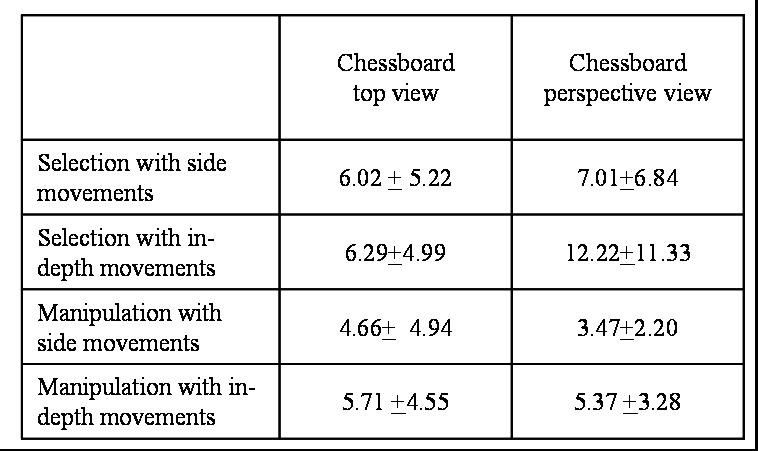
\includegraphics[width=.7\textwidth]{table.jpg}
% \end{table}

% \section{Images}

% All images and illustrations should be in black-and-white, or gray tones,
% excepting for the papers that will be electronically available (on CD-ROMs,
% internet, etc.). The image resolution on paper should be about 600 dpi for
% black-and-white images, and 150-300 dpi for grayscale images.  Do not include
% images with excessive resolution, as they may take hours to print, without any
% visible difference in the result. 

% \section{References}

% Bibliographic references must be unambiguous and uniform.  We recommend giving
% the author names references in brackets, e.g. \cite{knuth:84},
% \cite{boulic:91}, and \cite{smith:99}.

% The references must be listed using 12 point font size, with 6 points of space
% before each reference. The first line of each reference should not be
% indented, while the subsequent should be indented by 0.5 cm.

% \bibliographystyle{sbc}
% \bibliography{sbc-template}

\bibliographystyle{abnt}
\bibliography{sbc-template}

\end{document}